\documentclass[11pt]{amsart}
\usepackage{geometry}                % See geometry.pdf to learn the layout options. There are lots.
\geometry{letterpaper}                   % ... or a4paper or a5paper or ... 
%\geometry{landscape}                % Activate for for rotated page geometry
%\usepackage[parfill]{parskip}    % Activate to begin paragraphs with an empty line rather than an indent
\usepackage{graphicx}
\usepackage{amssymb}
\usepackage{epstopdf}
\usepackage{amsmath}
\usepackage{tikz}
\usepackage{subcaption}

\DeclareGraphicsRule{.tif}{png}{.png}{`convert #1 `dirname #1`/`basename #1 .tif`.png}
\usetikzlibrary{arrows,positioning}
% LB things
\newenvironment{packed_item}{
\begin{itemize}
 \setlength{\itemsep}{0pt}
  \setlength{\parskip}{0pt}
  \setlength{\parsep}{0pt}
}{\end{itemize}}

\newcommand{\Unif}{\text{Unif}}
\newcommand{\Beta}{\text{Beta}}
\newcommand{\Normal}{\text{Normal}}
\newcommand{\Binomial}{\text{Binomial}}
\newcommand{\E}{\mathbb{E}}
 
 




\title{Mechanistic Bayesian Forecasts of COVID19}
\author{Graham Gibson}
%\date{}                                           % Activate to display a given date or no date


\begin{document}
\section*{Abstract}
\begin{itemize}
\item Covid has affected XX people
\item Forecasts useful for public health resource planning, intervention planning (vaccine trials), and disease burden
\item Basic Mechanistic Models unable to capture complexities of real world disease epidemics due to 
\begin{itemize}
\item Complexities of interventions 
\item Issues with testing and reporting
\end{itemize}
\item We propose a novel forecasting algorithm to overcome 
\begin{itemize}
\item Under-reporting of cases
\item Time-varying interventions
\end{itemize}
\item Bayesian end to end estimation using both cases and deaths in numpyro
\end{itemize}


\maketitle

%\section{}
%\subsection{}

\section{Introduction}

\begin{itemize}
\item Emergence and spread of covid
\item Forecasts useful for public health
\begin{itemize}
\item Resource allocation
\item Intervention Planning
\item Disease burden
\end{itemize}
\item Cite Flu Forecasting
\item Describe COVID-HUB
\begin{itemize}
\item Number of participating teams as evidence of importance
\item Soliciting forecasts for incident and cumulative deaths
\end{itemize}
\item Mechanistic models have been around since K\&K
\item Demonstrated success in modeling infectious disease 
\item Since they were developed around the last pandemic their usefulness as applied forecasting models has gone untested
\item Extensions to basic model needed 
\begin{itemize}
\item Observations on cases and deaths
\item Time-varying detection probability for varied testing
\item Non-parametric model of interventions
\item Full Bayesian fitting due to unidentifiability of parameters given only a time series of cases and deaths.
\end{itemize}
\item MechBayes outperforms in two settings
\begin{itemize}
\item COVID-HUB relative to baseline model 
\item Ablation test relative to basic SEIR model
\end{itemize}
\item We show improvements in MAE and WIS relative to baseline model in both experimental setups

\end{itemize}

\section{Data}

\begin{itemize}
\item We use cases/deaths from JHU
\item Under-reporting issues
\item Batch reporting issues
\item Revision Issues
\item Weekly cycle issues
\item High variability in incident data
\item Ref Figure 1
\end{itemize}





 \begin{figure}
     \centering
     \includegraphics[scale=.1]{data_plot.png}
     \caption{Deaths by state. }
     \label{fig:my_label}
 \end{figure}
 
 \section{Compartmental Model}
 \begin{itemize}
 \item Basic SEIR model description
 \item Definition of compartmental model (description of diff eq as flow between compartments)
 \item Ref Figure 2
 \item Interpretation of parameters in basic SEIR model 
 \begin{itemize}
 \item Sigma
 \item Gamma
 \item beta
 \end{itemize}
 
 \end{itemize}
 
 \begin{figure}
     

 \begin{center}
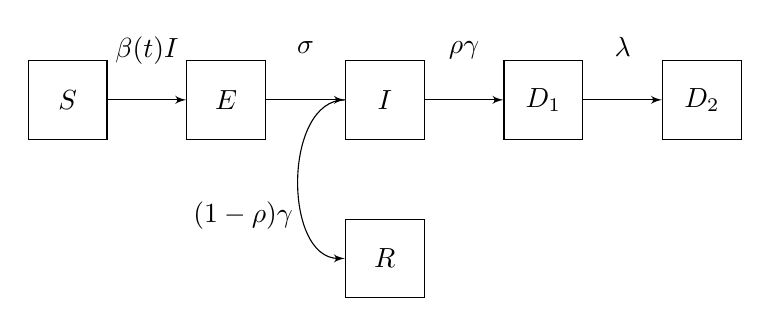
\begin{tikzpicture}[node distance=1cm,auto,>=latex',every node/.append style={align=center},int/.style={draw, minimum size=1cm}]
    \node [int] (S)             {$S$};
      \node [int,right=of S] (E)  {$E$};
    \node [int, right=of E] (I) {$I$};
    \node [int, right=of I] (D_1) {$D_1$};
    \node [int, right=of D_1] (D_2) {$D_2$};
     \node [int, below=of I] (R) {$R$};

   % \coordinate[right=of ] (out); %
    \path[->, auto=false] (S) edge node[yshift=12pt] {$\beta(t) I$ \\[.2em]} (E)
                          (E) edge node[yshift=12pt] {$\sigma$       \\[.2em] } (I) 
                           (I) edge node[yshift=12pt] {$\rho\gamma$       \\[.2em] } (D_1)
                           (I) edge[bend right=90] node[xshift=-20pt,yshift=-20pt] {$(1-\rho)\gamma$       \\[.4em] } (R)
                            (D_1) edge node[yshift=12pt] {$\lambda$       \\[.2em] } (D_2)  ;
                          \end{tikzpicture}
\end{center}
      \caption{Comparmental model parameters }
     \label{fig:seird}
 \end{figure}
 \subsection{Observations on cases and deaths}
 \begin{itemize}
 \item Bayesian model has observations on both cases and deaths
 \item We can weight likelihood of one over the other
 \item Explain how cases inform deaths on average 10 days later
 \end{itemize}
 
 \subsection{Time-varying beta parameter}
 \begin{itemize}
 \item Non-parametrically models time-varying transmissibility through a random walk
 \item Makes forecasts conditional on current level of interventions
 \item Requires no external intervention data to make forecasts 
 \item 
 \end{itemize}
 
 \subsection{Time-varying detection probability}
  \begin{itemize}
 \item Non-parametrically models time varying testing and overall detection of case issues
 \item Allows for "data dumps"
 \item Logistic random walk 
 \item Fixed detection probability on deaths

  \end{itemize}

\subsection{Seeding Epidemic}

 \begin{itemize}
 \item Because of detection probability we cannot seed using initial reported data, since this is an underestimate
 \item Put priors on initial seed
  \end{itemize}
  
  \subsection{Priors}

 \begin{itemize}
 \item We choose tight priors based on literature
  \item Fundamental unidentifiability due to renewal equation expression where $I(t)$ is a convolution between $R_t$ and Seiral interval
  \item Cannot estimate both simultaneously 
  \item Most flexibility comes in with beta and detection random walk
  \item Ideal for forecasting, maybe not for inference
  \end{itemize}
  
  \subsection{Fitting}

 \begin{itemize}
 \item Fully Bayesian HMC on parameters
 \item Why we choose deterministic compartmental model with only uncertainty on parameters and observations
 \item Estimation in numpyro very fast
   \end{itemize}
   
   
   
 \section{Experimental Setup}
 
 
 \subsection{COVID-HUB}
 \begin{itemize}
 \item Real-time forecasting evaluation for 14 weeks starting April 20th 2020. 
 \item Forecasts submitted every Monday using incident data up until Sunday
 \item Cumulative forecasts generated by aggregation of incident forecasts
 \item 1-4 week ahead targets generated from 28 day ahead predictions 
 \end{itemize}
 
 \subsection{Ablation Test}
 \begin{itemize}
 \item Evaluate a set of nested models
 \begin{itemize}
 \item Basic SEIR model with observations only on deaths
 \item SEIR with joint observations
 \item SEIR with joint observations and random walk detection probability
 \end{itemize}
 \item We omit the test that involves no random walk on beta since a model must take into account interventions.

 
 \end{itemize}


\section{COVID-Hub Results}


\begin{figure}
  \centering
     \begin{subfigure}{.5\textwidth}
  \centering
    \includegraphics[scale=.5]{US.png}
    \caption{US}
\end{subfigure}%
\begin{subfigure}{.5\textwidth}
  \centering
    \includegraphics[scale=.5]{NY.png}
    \caption{New York}
\end{subfigure}
\begin{subfigure}{.5\textwidth}
  \centering
    \includegraphics[scale=.5]{FL.png}
    \caption{Florida}
\end{subfigure}%
\begin{subfigure}{.5\textwidth}
  \centering
    \includegraphics[scale=.5]{CA.png}
    \caption{California}
\end{subfigure}%

\caption{Example fit and forecast for four states.}
\label{fig:fit_and_forecast_results}
\end{figure}

	
 \begin{figure}
     \centering
     \includegraphics[scale=.1]{beta_t_plot.png}
     \caption{Deaths by state. }
     \label{fig:my_label}
 \end{figure}
  \begin{figure}
     \centering
     \includegraphics[scale=.1]{detection_plot.png}
     \caption{Deaths by state. }
     \label{fig:my_label}
 \end{figure}
 
 

\begin{figure}
  \centering
     \begin{subfigure}{.5\textwidth}
  \centering
    \includegraphics[scale=.1]{mae_results_by_time_zero.png}
    \caption{MAE by timezero}
\end{subfigure}%
\begin{subfigure}{.5\textwidth}
  \centering
    \includegraphics[scale=.1]{mae_results_by_region.png}
    \caption{MAE by region}
\end{subfigure}
\begin{subfigure}{.5\textwidth}
  \centering
    \includegraphics[scale=.1]{wis_results_by_time_zero.png}
    \caption{WIS by timezero}
\end{subfigure}%
\begin{subfigure}{.5\textwidth}
  \centering
    \includegraphics[scale=.1]{wis_results_by_region.png}
    \caption{WIS by region}
\end{subfigure}%
\begin{subfigure}{.5\textwidth}
  \centering
    \includegraphics[scale=.1]{mae_results_by_target.png}
    \caption{WIS by timezero}
\end{subfigure}%
\begin{subfigure}{.5\textwidth}
  \centering
    \includegraphics[scale=.1]{wis_results_by_target.png}
    \caption{WIS by region}
\end{subfigure}%

\caption{Scores from covid-hub.}
\label{fig:covidhub}
\end{figure}



\begin{itemize}
\item MechBayes is almost always better than baseline model when broken down by region, target, and timezero after June 1st 2020.
\item MechBayes has improved over time.
\begin{itemize}
\item First two submissions did not have detection probability random walk
\item Observations were Normally distributed on cumulative deaths
\item Switched to current model
\end{itemize}
\item Naive baseline is hard to beat
\item MechBayes is biased high. This comes from uncertainty in the random walk leading to potentially huge growth rates. 
\end{itemize}   
   
   
   
   \section{Ablation Results}

   \begin{itemize}
   \item Model ranking is as follows
   \begin{itemize}
   \item MechBayes
   \item MechBayes-Case Observations
   \item MechBayes - no detection random walk
   \end{itemize}
   \item This ordering is inu
   \end{itemize}


\section{Discussion}
\begin{itemize}
\item Mech Bayes is a fast fully bayesian compartmental model capable of accounting for real-world modeling challenges during a pandemic.
\item Demonstrated success across regions, targets, and timezeros
\item Real-time model results show the practice of modeling during an epidemic. Results are improving.
\item Ablation studies show the results are grounded in real model improvements using historical validation.
\item Talk about how overall MAE obscures the huge geographic variability. 
\end{itemize}

\section{Conclusion}

\begin{itemize}
\item Summarize mech bayes as bayesian compartmental model
\item Further work: most of the model is about $\beta(t)$. Better methods for modeling it? Spline Etc.
\end{itemize}


\end{document}  
